\documentclass[a4paper]{article}
\usepackage[spanish]{babel}
\usepackage[utf8]{inputenc}
\usepackage{charter}   % tipografia
\usepackage{graphicx}


%%%%%%%LO AGREGUE%%%%%%%%%%  Y yo lo modifique
%\usepackage{hyperref}
%%%%%%%%%%%%%%%%%%%%%%%%%%

\usepackage[bookmarks = true, colorlinks=true, linkcolor = black, citecolor = black, menucolor = black, urlcolor = blue]{hyperref} 




%\usepackage{makeidx}
\usepackage{paralist} %itemize inline
\usepackage[ruled,vlined]{algorithm2e}
%\usepackage{float}
%\usepackage{amsmath, amsthm, amssymb}
%\usepackage{amsfonts}
%\usepackage{sectsty}
%\usepackage{charter}
%\usepackage{wrapfig}
%\usepackage{listings}
%\lstset{language=C}


\usepackage{color} % para snipets de codigo coloreados
\usepackage{fancybox}  % para el sbox de los snipets de codigo

\definecolor{litegrey}{gray}{0.94}

% \newenvironment{sidebar}{%
% 	\begin{Sbox}\begin{minipage}{.85\textwidth}}%
% 	{\end{minipage}\end{Sbox}%
% 		\begin{center}\setlength{\fboxsep}{6pt}%
% 		\shadowbox{\TheSbox}\end{center}}
% \newenvironment{warning}{%
% 	\begin{Sbox}\begin{minipage}{.85\textwidth}\sffamily\lite\small\RaggedRight}%
% 	{\end{minipage}\end{Sbox}%
% 		\begin{center}\setlength{\fboxsep}{6pt}%
% 		\colorbox{litegrey}{\TheSbox}\end{center}}

\newenvironment{codesnippet}{%
	\begin{Sbox}\begin{minipage}{\textwidth}\sffamily\small}%
	{\end{minipage}\end{Sbox}%
		\begin{center}%
		\vspace{-0.4cm}\colorbox{litegrey}{\TheSbox}\end{center}\vspace{0.3cm}}



\usepackage{fancyhdr}
\pagestyle{fancy}

%\renewcommand{\chaptermark}[1]{\markboth{#1}{}}
\renewcommand{\sectionmark}[1]{\markright{\thesection\ - #1}}

\fancyhf{}

\fancyhead[LO]{Sección \rightmark} % \thesection\ 
\fancyfoot[LO]{\small{Agustina Aldasoro, Francisco Noriega, Ezequiel Zimenspitz, Brian Zuker}}
\fancyfoot[RO]{\thepage}
\renewcommand{\headrulewidth}{0.5pt}
\renewcommand{\footrulewidth}{0.5pt}
\setlength{\hoffset}{-0.8in}
\setlength{\textwidth}{16cm}
%\setlength{\hoffset}{-1.1cm}
%\setlength{\textwidth}{16cm}
\setlength{\headsep}{0.5cm}
\setlength{\textheight}{25cm}
\setlength{\voffset}{-0.7in}
\setlength{\headwidth}{\textwidth}
\setlength{\headheight}{13.1pt}

\renewcommand{\baselinestretch}{1.1}  % line spacing


% \setcounter{secnumdepth}{2}
\usepackage{underscore}
\usepackage{caratula}
%\usepackage{url}
\usepackage{hyperref}

% ******************************************************** %
%              TEMPLATE DE INFORME ORGA2 v0.1              %
% ******************************************************** %
% ******************************************************** %
%                                                          %
% ALGUNOS PAQUETES REQUERIDOS (EN UBUNTU):                 %
% ========================================
%                                                          %
% texlive-latex-base                                       %
% texlive-latex-recommended                                %
% texlive-fonts-recommended                                %
% texlive-latex-extra?                                     %
% texlive-lang-spanish (en ubuntu 13.10)                   %
% texlive-science										  %
% ******************************************************** %



\begin{document}


\thispagestyle{empty}
\materia{Algoritmos y Estructuras de Datos III}
\submateria{Primer Cuatrimestre de 2015}
\titulo{Trabajo Práctico I}
%\subtitulo{subtitulo del trabajo}
\integrante{Aldasoro Agustina}{86/13}{agusaldasoro@gmail.com}
\integrante{Noriega Francisco}{660/12}{frannoriega.92@gmail.com}
\integrante{Zimenspitz Ezequiel}{155/13}{ezeqzim@gmail.com}
\integrante{Zuker Brian}{441/13}{brianzuker@gmail.com}


\maketitle
\newpage

\thispagestyle{empty}
\vfill
\begin{abstract}
Habi\'endonos sido dado una serie de tres problem\'aticas a resolver, se plantean sus respectivas soluciones acorde a los requisitos pedidos. Se adjunta una descripci\'on de cada problema y su soluci\'on, conjunto a su an\'alisis de correctitud y de complejidad sumado a su experimentaci\'on. El lenguaje elegido para llevar a cabo el trabajo es C++.

Estos son los comandos para compilar cada ejercicio (el flag se utiliz\'o para la librer\'ia <chrono> para medir tiempos de ejecucion):\\
	g++ -o main Zombieland.cpp -std=c++11\\
	g++ -o main AltaFrecuencia.cpp -std=c++11\\
	g++ -o main SenorCaballos.cpp -std=c++11
	
Dentro de cada .cpp est\'a el comando para compilar cada ejercicio desde la carpeta donde se encuentran los mismos.

\end{abstract}

\thispagestyle{empty}
\vspace{3cm}
\tableofcontents
\newpage


%\normalsize
\newpage
\section{Problema 1: ZombieLand}

\subsection{Descripci\'on de la problem\'atica}

En un pa\'is con \emph{n} ciudades, se encuentran una determinada cantidad de Zombies y de Soldados por cada una de ellas. El objetivo del problema es exterminar la invasi\'on zombie, para ello es necesario un enfrentamiento \textit{zombies vs soldados} por cada ciudad. Para que el combate sea positivo en una ciudad, es decir se logre matar a todos los zombies de la misma, es necesario que la cantidad de zombies sea, a lo sumo, diez veces m\'as grande que la cantidad de soldados.\\

Se sabe de antemano cu\'antos zombies y cu\'antos soldados se encuentran atrincherados en cada ciudad. Los soldados acuartelados no pueden moverse de la ciudad en la que est\'an, pero s\'i se cuenta con una dotaci\'on de soldados extra que se la puede ubicar en cualquiera de las \emph{n} ciudades para salvarla. La cantidad de soldados extra es ilimitada, mas los recursos para trasladarlos no lo son. El costo del traslado depende de cada ciudad. Siempre que se respete el presupuesto del pa\'is, se pueden trasladar todos los soldados necesarios para salvar a cada ciudad.\\

Debido a que los recursos econ\'omicos son finitos, no siempre va a ser posible salvar a las n ciudades. Lo que se desea en este problema es maximizar la cantidad de ciudades salvadas, respetando el presupuesto. Es decir, se deben establecer las cantidades de soldados extras enviados a cada ciudad de modo que la cantidad de ciudades salvadas sea la \'optima y gastando un monto por debajo del presupuesto.  El algoritmo debe tener una complejidad temporal de $O(n.log(n))$, siendo $n$ la cantidad de ciudades del pa\'is.\\

\textcolor{red}{Aca se podr\'ia poner unos dibujitos de soluciones \'optimas como para que quede m\'as lindo}


\newpage
\subsection{Resoluci\'on propuesta y justificaci\'on}

Para la resoluci\'on del problema decidimos utilizar un algoritmo goloso, que salvar\'a en cada paso a la ciudad que m\'as le convenga en ese momento, es decir, la que permita maximar la cantidad de ciudades salvadas.\\

Como primera instancia, el algoritmo simplemente calcula, para cada ciudad, cu\'anto ser\'ia el costo de salvarla. Para ello, primero se calcula la cantidad de soldados extra necesarios y luego se multiplica por el costo de traslado de cada unidad:\\


	\begin{codesnippet}
	\begin{verbatim}
		soldados_extras_necesarios = redondeo_hacia_arriba((zombies - (soldados_existentes * 10)) /10)
		
		costo_total = costo_unitario * soldados_extras_necesarios
	\end{verbatim}
	\end{codesnippet}

Luego de haber obtenido una magnitud con la cual se pueden comparar las ciudades entre s\'i, se ordenan las ciudades de menor a mayor en base al costo de salvarla para ser recorridas secuencialmente y enviar los ej\'ercitos requeridos hasta que se agote el presupuesto.\\

Notar que si alguna ciudad no requiere soldados extras para ser salvada, entonces ser\'an las primeras en ser salvadas dado que el costo_total ser\'a igual a 0.\\
 
Se recorren secuencialmente las ciudades ordenadas por el costo_total, de modo que para cada una se va a comparar el costo de salvarla contra el presupuesto restante en ese momento (presupuesto_actual). Si es factible el salvataje, se resta el costo_total del presupuesto_actual y se env\'ian las tropas necesarias a la ciudad; en caso contrario se la marca como ciudad perdida.\\

Vale aclarar que el orden impuesto a las ciudades implica que cuando ya no se pueda salvar a una ciudad, no se podr\'a salvar a ninguna otra de las restantes.\\
 
%Como en este vector las ciudades no aparecen en orden creciente por su n\'umero, debemos reordenarlas. Debido a que el \emph{id} de cada ciudad va a ser \'unico y va a encontrarse en el intervalo [0, n-1], se lo recorre secuencialmente colocando cada ciudad en la posici\'on de su \textit{id} dentro de un nuevo vector \emph{respuesta} . \textcolor{red}{Ver que este parrafo me aprece que no quedo muy claro...} \textcolor{blue}{es necesario este p\'arrafo? habla del stdout... no me parece necesario en absoluto... yo lo sacar\'ia}\\

A continuación demostraremos que el algoritmo resuelve efectivamente el problema planteado.\\

\textbf{Teorema}
El algoritmo resuelve el problema planteado, salvando la mayor cantidad de ciudades posibles.\\

\textbf{Demostraci\'on}
Para demostrar el teorema enunciado, supondremos que nuestro algoritmo no devuelve una solución óptima, y tomaremos la solución óptima con más ciudades salvadas en común.
Sean $C_{k}$ las ciudades de la solución óptima y $D_{k}$ las ciudades de la solución dada por el algoritmo, y supondremos que están ordenadas de menor a mayor, según el costo de ser salvadas.
Sea $C_{j}$ la primer ciudad distinta a las ciudades de $D$, de modo que $C_{i}$ = $D_{i}$ $\forall i, i < j$.\\

Entonces, hasta $C_{i-1}$, el costo total por salvar dichas ciudades es el mismo al de $D$ hasta $D_{i-1}$. Pero ya que el algoritmo elige siempre la ciudad que (pudiendo salvarse) cueste lo menor posible, eso significa que $C_{i}$ tiene un costo igual o mayor al de $D_{i}$, con lo cual si en $C$ reemplazamos $C_{i}$ por $D_{i}$, seguimos teniendo presupuesto (en particular, mayor que el que se tenía) y se salvan la misma cantidad de ciudades, por lo que debe ser óptimo.\\

Pero esta nueva solución, es una solución óptima que tiene más ciudades en común que $C$, por lo que es absurdo, ya que $C$ era la solución óptima que más ciudades en común tenía con $D$.\\

El absurdo proviene de suponer que $D$ no es óptimo y que por lo tanto la solución óptima con más ciudades salvadas en común con $D$, no es $D$.\\

Así, $D$ debe ser óptimo, en el sentido de que debe tener la mayor cantidad ciudades que pueden ser salvadas, para el presupuesto y costos para cada ciudad dados.

\newpage
\subsection{An\'alisis de la complejidad}
La complejidad de nuestra soluci\'on es $O(n.log(n))$, siendo \emph{n} la cantidad de ciudades del pa\'is.\\

En primera instancia, guardamos los datos de las ciudades pasadas por stdin en structs y los dejamos dentro de un vector, para luego poder utilizarlas de un modo pr\'actico. Como esto se realiza secuencialmente, tiene costo lineal \textbf{\textit{O(n)}}.

\begin{algorithm}[h!]
\caption{zombieland}
\For{\emph{each} ciudad $\in$ pa\'is}{
	Calcular la cantidad de soldados extra necesarios y el costo de salvarla.\\
	Almacenar esta informaci\'on en un vector \emph{datos} mediante \textit{push_back()}
}
Ordena al vector \emph{datos} mediante \textit{sort()}\\
\While{pueda salvar}{
	\If{puede ser salvada}{
		Indicar cantidad de soldados extras enviados y actualizar el presupuesto_actual
	}
}
\While{haya ciudades insalvables}{
	cantidad de soldados extras enviados = 0
}
\textcolor{blue}{es necesario este cacho? habla del stdout... no me parece necesario en absoluto... yo lo sacar\'ia}\\
\For{\emph{each} ciudad \emph{en vector} datos}{
	Insertar en el vector \emph{respuesta}[ciudad.id] la ciudad actual. 
}
\end{algorithm}
\textcolor{red}{En el codigo, yo pondria este reordenamiento dentro de zombieland, ya que hay que considerarlo para medir tiempos.}\\
\textcolor{blue}{A mi no me parece que sea necesario para medir tiempos... o sea, arrancar de la instancia pasada por parametro, salvo que la limemos y usemos avls, heaps, etc. no me parece necesario contarlas. lo mismo para escribir, la respuesta est\'a, en el ej2 tenemos que calcular un pedazo de respuesta post algoritmo y lo hacemos y lo consideramos, el std out extra porque deber\'iamos considerarlo? es algo que nos piden para visualizar, si las cosas andan mal, porque pueden llegar a estar mal}\\

\textcolor{red}{Dijo el ayudante que eso si habia que ponerlo....}

El c\'odigo presenta un \textbf{primer ciclo \emph{for}} que calcula el costo de salvar a cada ciudad y las agrega mediante push_back() a un vector. El ciclo recorre linealmente todas las ciudades por lo que tiene complejidad $O(n)$. 

El c\'alculo de salvar a cada ciudad coincide con el descripto en la secci\'on anterior, el cual por ser operaciones aritm\'eticas es $O(1)$. Armar el nuevo struct para insertar dentro del vector \emph{datos} tambi\'en posee un costo constante $O(1)$. La funci\'on \href{http://www.cplusplus.com/reference/vector/vector/push_back/}{push\_back()} \footnote{http://www.cplusplus.com/reference/vector/vector/push_back/} tiene costo $O(1)$ amortizado, lo que implica que cuando no precisa redimensionar el vector cuesta esto, y cuando lo hace, toma tiempo lineal en la cantidad de elementos. Como insertamos durante todo el ciclo tomamos el costo amortizado $O(1)$.
Por lo tanto, la complejidad total del primer ciclo for nos da \textbf{\textit{O(n)}}.\\

Le sigue \textbf{ordenar el vector} con estos datos, para ello usamos \href{http://www.cplusplus.com/reference/algorithm/sort/}{sort()} \footnote{http://www.cplusplus.com/reference/algorithm/sort/} cuya complejidad es \textbf{\textit{O(n.log(n)})}.\\

A continuaci\'on, se realizan dos \textbf{\'ultimo ciclos \emph{while}} el primero salva todas las ciudades que pueda, mientras dure el presupuesto y el segundo deja en \emph{0 soldados enviados} a las ciudades que no pueden ser salvadas. Estos c\'alculos aritm\'eticos y asignaciones son todos de complejidad constante $O(1)$. El primer ciclo toma $O(ciudades\_salvadas)$ y el segundo $O(n-ciudades\_salvadas)$ dando como resultado un recorrido lineal sobre todas las ciudades, por lo tanto lo hace con complejidad \textbf{\textit{O(n)}}.\\

\textcolor{blue}{Para mi no va...}\textcolor{red}{Dijo que siiiiii}\\

Finalmente, se debe \textbf{reordenar el vector} obtenido hasta ahora para que quede en orden creciente respecto de su \textit{id}. Como esto se hace recorriendo secuencialmente el primer vector, asign\'andole uno a uno los elementos al nuevo vector \emph{respuesta} indexados; s\'olo hace una pasada lineal con costo \textbf{\textit{O(n)}}.\\

Como cada paso de los mencionados son secuenciales, las complejidades se suman, obteniendo:\\

$O(n)$ + $O(n.log(n))$ + $O(n)$ 
% + $O(n)$
 que es igual a \textit{\textbf{O(n.log(n))}} por propiedades de $O$.


\newpage

\subsection{C\'odigo fuente}

	\begin{codesnippet}
	\begin{verbatim}
struct ciudad{
    int zombies;
    int soldados;
    int costo;
};
	\end{verbatim}
	\end{codesnippet}

	\begin{codesnippet}
	\begin{verbatim}
struct ciudad2{
    int numCiudad;
    int soldadosNecesarios;
    int costoTotal;
    bool operator< (const ciudad2& otro) const{
        return costoTotal < otro.costoTotal;
    }
};
	\end{verbatim}
	\end{codesnippet}


	\begin{codesnippet}
	\begin{verbatim}
int main(int argc, char const *argv[]){
    chrono::time_point<chrono::system_clock> start, end;
    long int cantCiudades, presupuesto;
    vector<ciudad> pais;
//Leemos informacion del problema
    cin >> cantCiudades;
    cin >> presupuesto;
    for (int i = 0; i < cantCiudades; ++i){
        ciudad alguna;
        cin >> alguna.zombies;
        cin >> alguna.soldados;
        cin >> alguna.costo;
        pais.push_back(alguna);
    }
    long int salvadas = 0;
    start = chrono::system_clock::now();
//Aplicamos el algoritmo
    vector<ciudad2> res = zombieland(cantCiudades, presupuesto, pais, salvadas);
    end = chrono::system_clock::now();
    vector<long int> entregados(cantCiudades);
//Stdout pedido
    for (int i = 0; i < cantCiudades; ++i){
        entregados[res[i].numCiudad] = res[i].soldadosNecesarios;
    }
    cout << salvadas << " ";
    for (int i = 0; i < cantCiudades; ++i){
        cout << entregados[i] << " ";
    }
    cout << endl;
    chrono::duration<double> elapsed_seconds = end-start;
    cout << "Tiempo: " << elapsed_seconds.count() << endl;
    return 0;
}
	\end{verbatim}
	\end{codesnippet}
	
	
	\begin{codesnippet}
	\begin{verbatim}
const vector<ciudad2> zombieland(long int cantCiudades, long int presupuesto, 
const vector<ciudad>& pais, long int& salvadas){
    salvadas = 0;
    vector<ciudad2> datos;
    for (int i = 0; i < cantCiudades; ++i){
        ciudad2 actual;
//ID de la ciudad
        actual.numCiudad = i;
//Calculamos el costo de salvar la ciudad i
        double diferencia = (pais[i].zombies - pais[i].soldados * 10);
        if (diferencia > 0)
            actual.soldadosNecesarios = ceil(diferencia/10);
        else
            actual.soldadosNecesarios = 0;
        actual.costoTotal = actual.soldadosNecesarios * pais[i].costo;
//Lo agregamos al vector
        datos.push_back(actual);
    }
//Ordenamos el vector de menor a mayor costo para salvarlas
    sort(datos.begin(), datos.end());
    long int dif = presupuesto;
//Vemos cuantas salvamos respetando el presupuesto
    int i = 0;
    while(i<cantCiudades && dif >= 0){
        dif = presupuesto - datos[i].costoTotal;
        if (dif>=0){
            salvadas++;
            presupuesto = dif;
            ++i;
        }
    }
//Las que sobran no se salvan
//seteamos los soldados necesarios en 0 para imprimir una respuesta correcta
    while(i<cantCiudades){
        datos[i].soldadosNecesarios = 0;
        ++i;
    }
    return datos;
}
	\end{verbatim}
	\end{codesnippet}
\newpage
\subsection{Experimentaci\'on}

\subsubsection*{Constrastaci\'on Emp\'irica de la complejidad}



 


%%%%%%%%%%%%%%%%%%%%%%%%%%%%%%%%%%%%%%%%%%%%%%%%%%%%%%%%%%%%%%%%%%%%%%%%%%%%%%%%%%%%%%%%%%%%%%%%%%%%%%%%%%%%%
%\newpage
%\subsubsection{Modificaci\'on del algoritmo}

%Decidimos hacer una modificaci\'on dentro del algoritmo. Creemos que esta misma va a generar una mejora en la cantidad de tiempo.\\

%La misma consiste en: modificar el \'ultimo \emph{ciclo for} para que cuando encuentre la primer ciudad que no pueda salvar deje de iterar ya que las restantes tampoco podr\'an ser salvadas (esto ocurre porque est\'an ordenadas por costo).\\

%Consideramos que saliendo antes del ciclo, el tiempo de c\'omputo para un mismo pa\'is deber\'ia ser menor que con el algoritmo original.\\

%Experimentamos 10 casos distintos de tama\~no 1000\textcolor{red}{(?} y para cada uno comparamos sus tiempos de ejecuci\'on entre el algoritmo original y el modificado.

%\textcolor{red}{Aca va el gr\'afico de eso que acabo de explicar arriba.}

%\newpage
%\subsubsection{Comparar pa\'ises de a dos}

%Consideramos 10\textcolor{red}{??} casos, donde para cada uno tomamos dos paises (A y B) con la misma cantidad de ciudades \textcolor{red}{para cada par de paises, cantidades distintas de ciudades (100, 500, 1000, ... (hasta donde nos de la compu jajaj))}. Estos casos los vamos a armar de tal forma que A tenga ya todas sus ciudades salvadas al momento de ser ingresada, en cambio B tiene una relaci\'on de cantidad soldados/zombies aleatoria. Corremos el algoritmo para todos los pares de paises.\\

%Dado a que nuestro algoritmo no establece ning\'un control de filtro sobre casos donde las ciudades ya esten salvadas al momento de ser recibidas como par\'ametro, consideramos que para cada par de ciudades los tiempos de c\'omputo no van a diferir mucho.\\

%\textcolor{red}{Aca va el gr\'afico donde muestra la diferencia entre cada par. Y ver si lo dibujamos linealizado como mostraron en clase tambien.}\\

%\textcolor{red}{Aca hay que escribir si coincidi\'o con lo que creiamos o no y dar una peque\~na explicaci\'on de porque pasa eso}


%\noindent Experimentos que se pueden hacer:
%-Muchas ciudades con pocos soldados para mandar, pero presupuesto bajo. Hipotesis: realmente es la cantidad optima, sin importar la que elija.

\newpage
\section{Problema 2: Alta Frecuencia}
\subsection{Descripci\'on de la problem\'atica}

Se quiere transmitir informaci\'on secuencialmente mediante un enlace el mayor tiempo posible. Los enlaces tienen asociadas distintas frecuencias, con un costo por minuto y un intervalo de tiempo (sin cortes) en el cual funcionan. Se utilizan durante minutos enteros, y es posible cambiar de una frecuencia a otra instant\'anemente (del minuto 1 al 4 uso la frecuencia A y del 4 al 6 la B). Los datos del precio y e intervalo de tiempo de cada frecuencia son dados. Se desea optimizar este problema para transmitir todo el tiempo que tenga al menos una frecuencia abierta, pero gastando la menor cantidad de dinero. Se debe contar con una complejidad de $O(n.log(n))$.\\

A continuaci\'on se muestran dos casos particulares de este problema. En ambos se ofrecen tres frecuencias, con distintos costos cada una. Se puede ver recuadrado en violeta cu\'al es la elecci\'on que debe hacerse por intervalo de tiempo.


 \begin{figure}[h!]
   \begin{center}
 	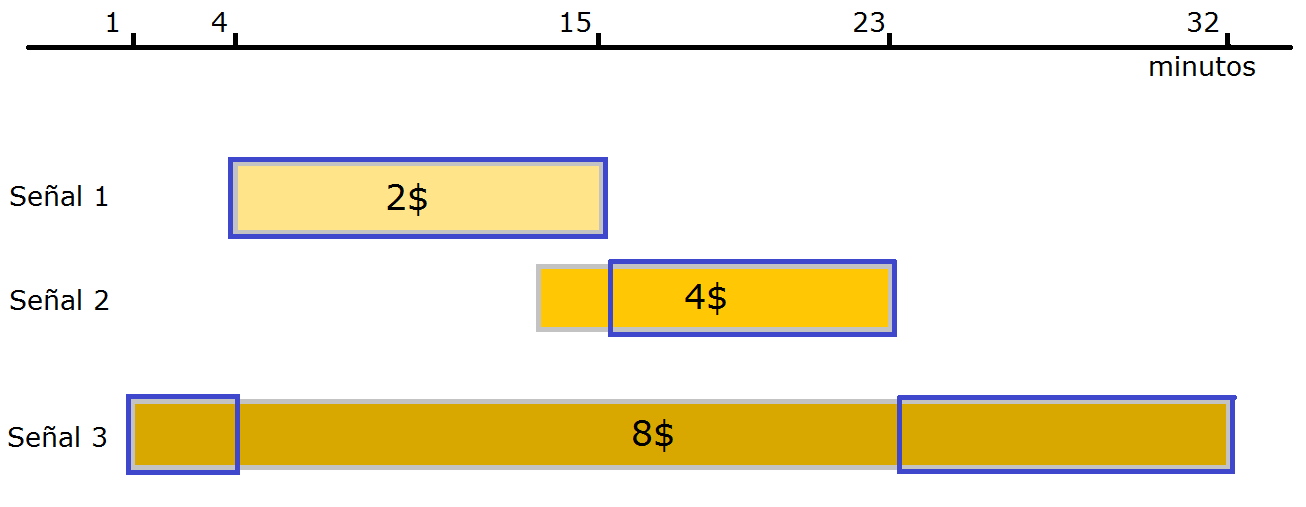
\includegraphics[scale=0.45]{imagenes/ej2/ejemplo1.png}
 	\caption{Ejemplo 1}
% 	\label{caballito}	
   \end{center}
 \end{figure}

 \begin{figure}[h!]
   \begin{center}
 	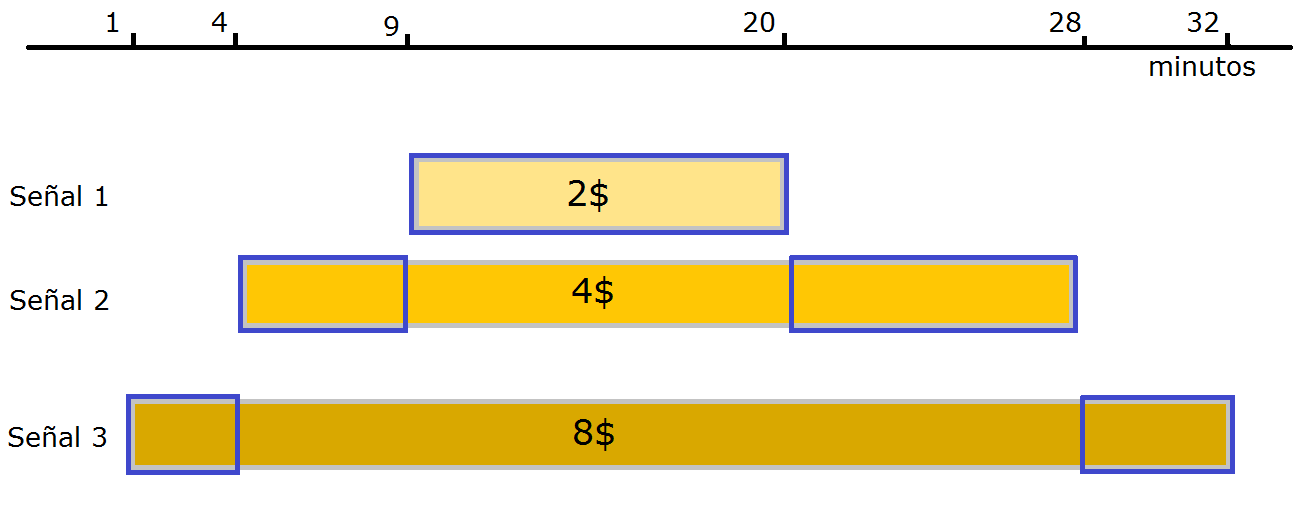
\includegraphics[scale=0.45]{imagenes/ej2/ejemplo2.png}
 	\caption{Ejemplo 2}
% 	\label{caballito}	
   \end{center}
 \end{figure}


\newpage

\subsection{Resoluci\'on propuesta y justificaci\'on}

El algoritmo que utilizamos pertenece a la familia de \emph{Divide \& Conquer}.\\

%\textcolor{red}{Aca pasa lo mismo de la implementacion porque hablamos mucho de vector y bla...}\\

El primer paso consiste en ordenar las frecuencias de menor a mayor en base al costo de cada una.\\

Luego, se sigue el esquema cl\'asico de Divide \& Conquer:\\

	\begin{codesnippet}
	\begin{verbatim}
divide(conjuntoDeFrecuencias F){
    Si hay mas de un elemento:
        Divido F en mitades A, B.
        intervalosA = divide(A)
        intervalosB = divide(B)
        Devuelvo conquer(intervalosA, intervalosB)
    Si hay un solo elemento:
        Lo devuelvo.	
}
	\end{verbatim}
	\end{codesnippet}

En palabras, si hay una sola frecuencia, la devolvemos, pues es trivial que su intervalo de duraci\'on es el m\'as barato y el de mayor extensi\'on temporal.\\

Si no, intervalosA ser\'a el conjunto de intervalos en la que funcionar\'a cada frecuencia, de modo que el costo de contratar el servicio con este cronograma sea m\'inimo en el costo y m\'aximo en la cantidad de tiempo de uso. E intervalosB ser\'a un conjunto con las mismas carater\'isticas, con la diferencia de que el A ser\'a el m\'as \'optimo de la mitad m\'as barata y el B el m\'as \'optimo de la mitad m\'as cara. Esto resulta de haber ordenado las frecuencias por su costo antes de comenzas con este tramo de algoritmo.\textcolor{red}{No se si este parrafo se entiende mucho}\\

Al hacer conquer(intervalosA, intervalosB) se obtiene el conjunto de intervalos con las caracter\'isticas mencionadas pero de todas las frecuencias.\textcolor{red}{No habria que explicar mas aca?}\\

%Nuestro algoritmo de Merge (\emph{conquer}) se encarga de elegir entre las frecuencias de dos arreglos pasados como parámetro, de modo que devuelve un sólo vector indicando los intervalos ocupados por las frecuencias elegidas. 

%Dado el enunciado del problema, para elegir qu\'e frecuencia utilizar en determinado intervalo de tiempo se debe priorizar el precio m\'as barato emitiendo se\~nal siempre que sea posible.\\

%Gracias a que en el primer llamado de nuestra funci\'on estas se encontraban en orden creciente respecto del costo, en cada paso de \emph{conquer} de los dos arreglos de entrada con intervalos se van a priorizar los de la izquierda. Es decir que en cada paso, todos los intervalos pertenecientes al vector de la izquierda (como son los de menor precio) van a pertencer al vector resultado. Mientras que s\'olo los intervalos que completen tiempo sin se\~nal pertenecientes al vector de la derecha van a ser colocados en el vector resultado. Esto representa un invariante que se va a cumplir en cada paso del algoritmo, lo cual nos permite justificar que la soluci\'on obtenida es la deseada. \textcolor{red}{Que alguien lea esto para ver si se entiende, para mi si :)}\\

%	\begin{codesnippet}
%	\begin{verbatim}
%conquer(conjuntoDeFrecuencias A, conjuntoDeFrecuencias B){
%	vector<frecuencia>::iterator iterCara = cara.begin(), iterBarata = barata.begin();
%	vector<frecuencia> res;
%	
%	En el conjunto res voy a tener el resultado.
%    Voy recorriendo en orden A y B, mientras haya elementos en A:
%    //Llamo A[i] al intervalo actual de A y B[j] al de B.
%        Si B[j] comienza antes que A[i]:
%            Si B[j] termina antes que A[i]:
%                Inserto B[j] en res.
%                j++
%            Si B[j] termina despues que A[i] empiece                                                                                                                                                                                                                                                                                                                                                                                                                                                                                                                                                                                                                                                                                                                                                                                                                                                                                                                                                                                                                                                                                                                                                                                                                                                                                                                                                              :
%                
%    
%    
%        Si A[i] comienza antes que B[j]:
%            Inserto A[i] en res
%            Si B[j] se superpone en algun momento con A[i]:
%                Al comienzo de B[j] le asigno el final de A[i]
%
%
%
%
%	while(iterCara != cara.end()){
%		if(iterBarata != barata.end()){
%			if(iterCara->principio < iterBarata->principio){ //la cara empieza antes
%				if(iterCara->fin <= iterBarata->principio){ //la cara termina antes de que empiece la barata
%					res.push_back(*iterCara);				//meto la cara entera
%					iterCara++;
%				}
%				else{ //la cara empieza antes y termina despues del principio de la barata
%					frecuencia antes;
%					antes.id = iterCara->id;
%					antes.costo = iterCara->costo;
%					antes.principio = iterCara->principio;
%					antes.fin = iterBarata->principio;
%					res.push_back(antes);
%					iterCara->principio = iterBarata->fin;
%				}
%			}
%			else{ //la barata empieza antes (o igual) que la cara
%				if(iterCara->fin > iterBarata->fin){ //la cara termina despues que la barata
%					if (iterCara->principio < iterBarata->fin) //este if es nuevo
%						iterCara->principio = iterBarata->fin;
%					res.push_back(*iterBarata);
%					iterBarata++;
%				}
%				else
%					iterCara++;
%			}
%		}
%		else{
%			if(iterCara->principio < iterCara->fin)
%				res.push_back(*iterCara);
%			iterCara++;
%		}
%	}
%	while(iterBarata != barata.end()){
%		res.push_back(*iterBarata);
%		iterBarata++;
%	}
%	return res;
%}
%
%	\end{verbatim}
%	\end{codesnippet}

Este \'ultimo paso abusa del invariante: todos los intervalos del conjunto intervalosA deben aparecer en el conjunto soluci\'on, y que lo \'unico que debe agregar son los intervalos de intervalosB que o bien aumentan el rango de tiempo para transmitir (uso el servicio desde antes o m\'as tiempo) o bien completan gaps que puedan existir entre las frecuencias m\'as baratas.

%Este algoritmo resuelve lo propuesto dando una soluci\'on \'optima porque del modo en que est\'a definido, primero divide al grupo con todas las frecuencias ofrecidas recursivamente hasta llegar a conjuntos con una sola frecuencia. Luego, al momento de mergear estos grupos de a dos, siempre prioriza al grupo de la izquierda (el m\'as barato). 

%Esto quiere decir que en el primer paso de este \textit{merge} se van a comparar solamente dos frecuencias entre s\'i, colocando la frecuencia m\'as barata completa y; si la oferta de intervalos de la frecuencia m\'as cara completa uno o dos intervalos donde no se le hab\'ia asignado se\~nal, se le otorga a ellos la frecuencia m\'as cara. De este modo, comparamos de a dos, frecuencias consecutivas otorg\'andole prioridad a la frecuencia m\'as barata. \textcolor{red}{Poner dibujito.} 

%En el siguiente paso del \textit{merge} se van a comparar dos conjuntos de intervalos con dos frecuencias en cada uno. Cada uno de estos conjuntos puede estar conformado por uno, dos o tres intervalos. \textcolor{red}{Poner dibujito} Gracias al formato de nuestro algoritmo, en cada paso del merge se preserva el invariante de que el conjunto ubicado a la izquierda tiene las frecuencias m\'as baratas mientras que el de la derecha tiene las m\'as caras. Se prosigue de manera an\'aloga a lo anterior, se preservan todos los intervalos de frecuencias pertenecientes al conjunto de los m\'as baratos y s\'olo se agregan frecuencias del conjunto caro en caso de que esten disponibles en intervalos de tiempos que hayan quedado vac\'ios.

%Estos pasos se van a reiterar, comparando conjuntos de intervalos entre dos, hasta que se hayan recorrido todas las frecuencias.\\

%Una vez terminados todos los pasos recursivos, vamos a contar con el conjunto de intervalos que completen la mayor cantidad de tiempo con el costo m\'as bajo. Si no hay dos frecuencias con el mismo costo, esta soluci\'on (\'optima) es \'unica, en caso contrario podr\'ia existir m\'as de una soluci\'on \'optima. \\

\newpage

\subsection{An\'alisis de la complejidad}

Para realizar este análisis primero es necesario calcular cu\'antos intervalos contendr\'a, como m\'aximo, el conjunto soluci\'on (desde ahora ``\emph{CS}''). Este valor ser\'a $2n-1$, siendo $n$ la cantidad de frecuencias dadas como par\'ametro.

Esto se deduce de analizar las posibles entradas para el algoritmo. Primero vamos a analizar el caso donde no existan dos frecuencias pasadas como par\'ametro con el mismo valor. De este modo la soluci\'on \'optima al problema va a ser \'unica. \\


Supongamos \textbf{n=1}. El intervalo de la frecuencia pasada como par\'ametro ser\'a el \'unico elemento del \emph{CS} y verifica $2n-1$ $=$ $2$.$1-1$ $=$ $1$.\\

Luego, tomamos \textbf{n=2}. De este modo, ambas pueden solaparse o ser disjuntas. Llamamos $1$ a la frecuencia m\'as barata y $2$ a la m\'as cara, $1$ va a estar incluida completa en \emph{CS} y $2$ puede formar dos intervalos, uno o ninguno. A continuaci\'on, se adjuntan cada uno de los casos, indicando en naranja los intervalos que pertenecer\'an a \emph{CS}.\\

La frecuencia $2$ no forma ning\'un intervalo:

 \begin{figure}[h!]
   \begin{center}
 	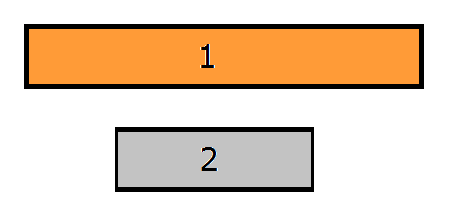
\includegraphics[scale=0.45]{imagenes/ej2/secuencias/Paso1/Caso0.png}
% 	\caption{}
% 	\label{caballito}	
   \end{center}
 \end{figure}

La frecuencia $2$ forma un intervalo:

 \begin{figure}[h!]
   \begin{center}
 	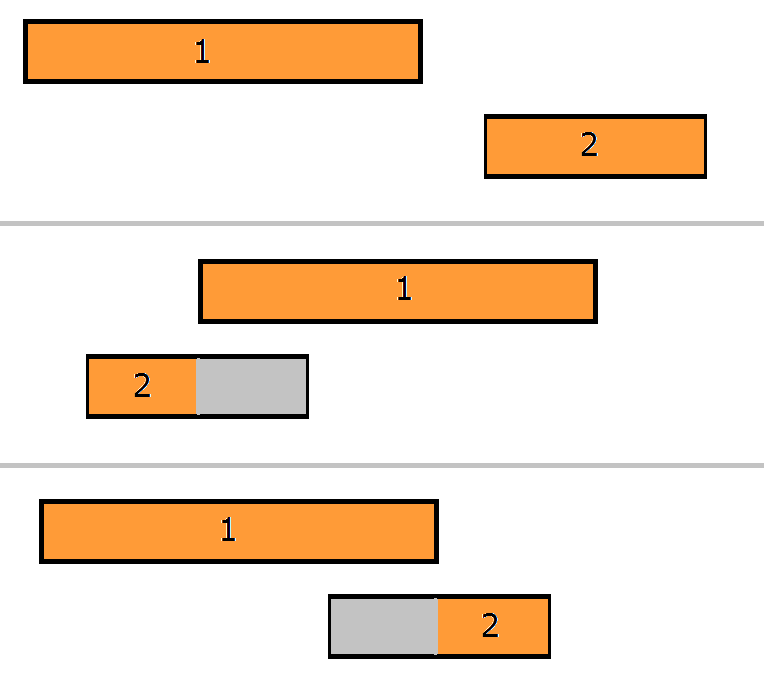
\includegraphics[scale=0.45]{imagenes/ej2/secuencias/Paso1/Caso1.png}
% 	\caption{}
% 	\label{caballito}	
   \end{center}
 \end{figure}
 

 \newpage
La frecuencia $2$ forma dos intervalos: 
 
  \begin{figure}[h!]
   \begin{center}
 	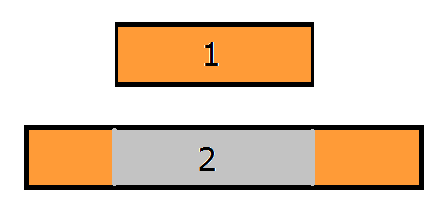
\includegraphics[scale=0.45]{imagenes/ej2/secuencias/Paso1/Caso2.png}
% 	\caption{}
% 	\label{caballito}	
   \end{center}
 \end{figure}
 


Es decir, para n=2 la cantidad m\'axima de intervalos posibles es $3$ intervalos, lo cual tambi\'en cumple $2n-1$ $=$ $2$.$2-1$ $=$ $3$.\\
 
%, entonces dado una frecuencia (la m\'as barata), la otra (m\'as cara) puede que se solape o no. Si no lo hace, entonces el CS tendr\'a ambos intervalos incluidos. Si se solapa, 1) est\'a inclu \'ido, con lo cual el CS ser\'a contendr\'a solo a la primer frecuencia; 2) arranca o termina mientras la otra est\'a disponible, dejando al CS con \'unicamente el pedazo de intervalo que no se solapa y el otro entero; o bien 3) arranca y termina antes y despu\'es de que arranque y termina el primero, logrando que el CS tenga un primer intervalo de la segunda frecuencia, hasta que arranca la primera, que entra por completo y luego un segundo intervalo de la segunda frecuencia que empieza cuando termina la primera. Esto se extiende para todo n con los mismos resultados, solo que puede agregarse un 4) completar un gap.\\

Al momento de tomar \textbf{n=3}, lo hacemos considerando las frecuencias $1$, $2$ y $3$. Partimos del caso anterior al que le a\~nadimos la frecuencia $3$. Es decir, vamos a contar con a lo sumo $3$ intervalos. La distribuci\'on de los intervalos se va a dar de la siguiente manera:\\

  \begin{figure}[h!]
   \begin{center}
 	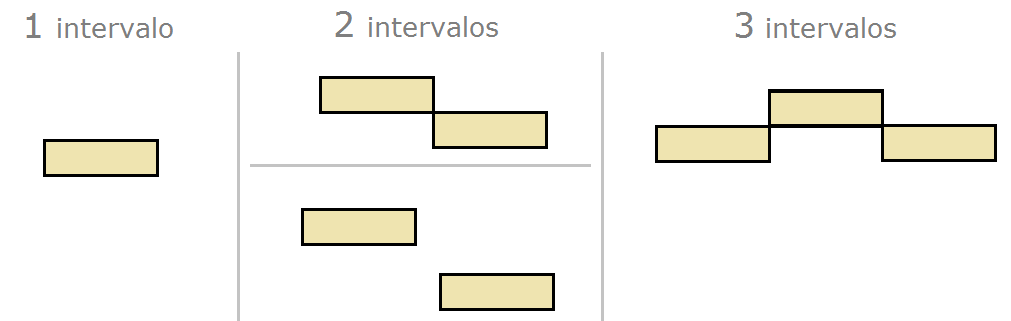
\includegraphics[scale=0.45]{imagenes/ej2/secuencias/salida2.png}
% 	\caption{}
% 	\label{caballito}	
   \end{center}
 \end{figure}

Podemos observar que de las cuatro distribuciones distintas que pueden ocurrir, en s\'olo una los intervalos son completamente disjuntos, esto es en el caso donde se a\~nadi\'o el intervalo $2$ completo. En los dem\'as casos, si bien pueden ser uno, dos o tres intervalos distintos al unirlos conforman un intervalo continuo, por lo cual entre ellos no va a haber gaps, es decir s\'olo se podr\'an a\~nadir intervalos en los bordes. Por este motivo, a estos casos los tomamos an\'alogos al caso de $n=2$ donde se agregar\'an a lo sumo dos intervalos, lo cual conforma en el caso m\'aximo 3 intervalos pre-existentes y 2 nuevos, dando un total de 5. Esto cumple lo planteado $2n-1$ $=$ $2$.$3-1$ $=$ $5$.\\

Ahora debemos considerar por separado, el caso donde contamos con dos intervalos pre-existentes totalmente disjuntos.\\

El \'unico caso donde se adicionan tres intervalos es el siguiente:\\
  \begin{figure}[h!]
   \begin{center}
 	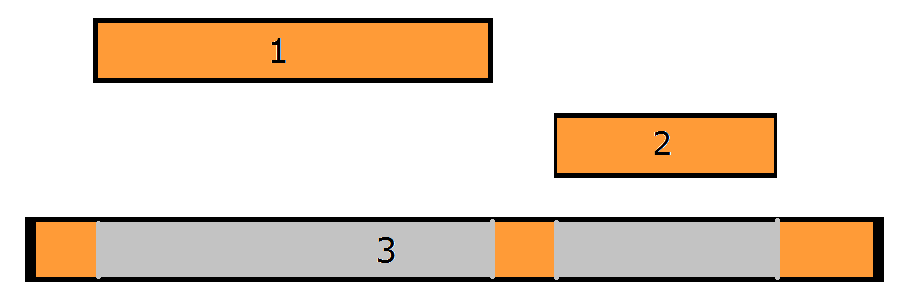
\includegraphics[scale=0.45]{imagenes/ej2/secuencias/Paso2/Caso3.png}
% 	\caption{}
% 	\label{caballito}	
   \end{center}
 \end{figure}
\newpage

Los casos donde se adicionan dos intervalos son los mostrados a continuaci\'on:
  \begin{figure}[h!]
   \begin{center}
 	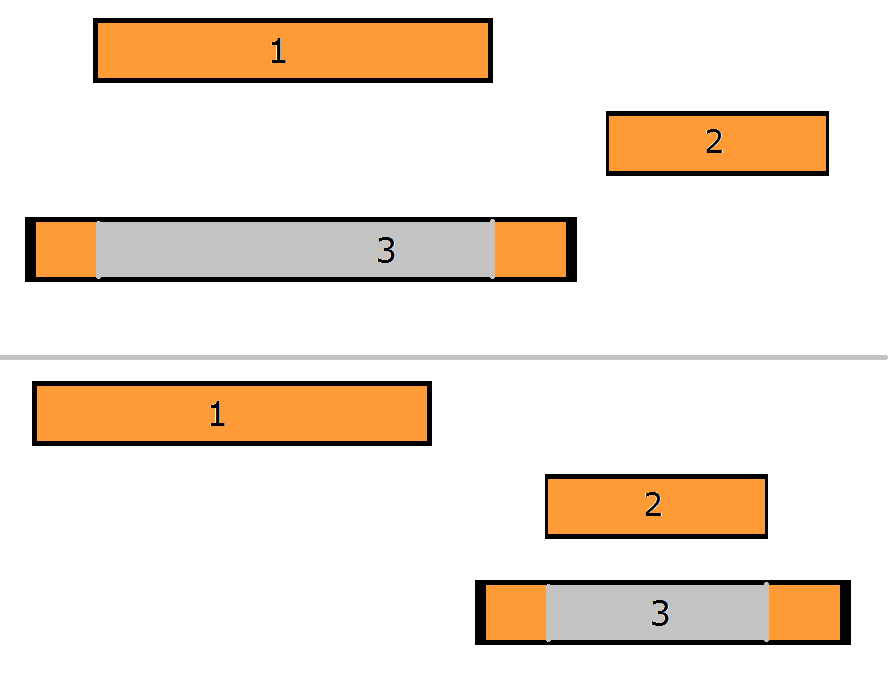
\includegraphics[scale=0.45]{imagenes/ej2/secuencias/Paso2/todos2.png}
% 	\caption{}
% 	\label{caballito}	
   \end{center}
 \end{figure}


Los siguientes son los casos donde al agregar la frecuencia $3$ s\'olo se adiciona un intervalo:
  \begin{figure}[h!]
   \begin{center}
 	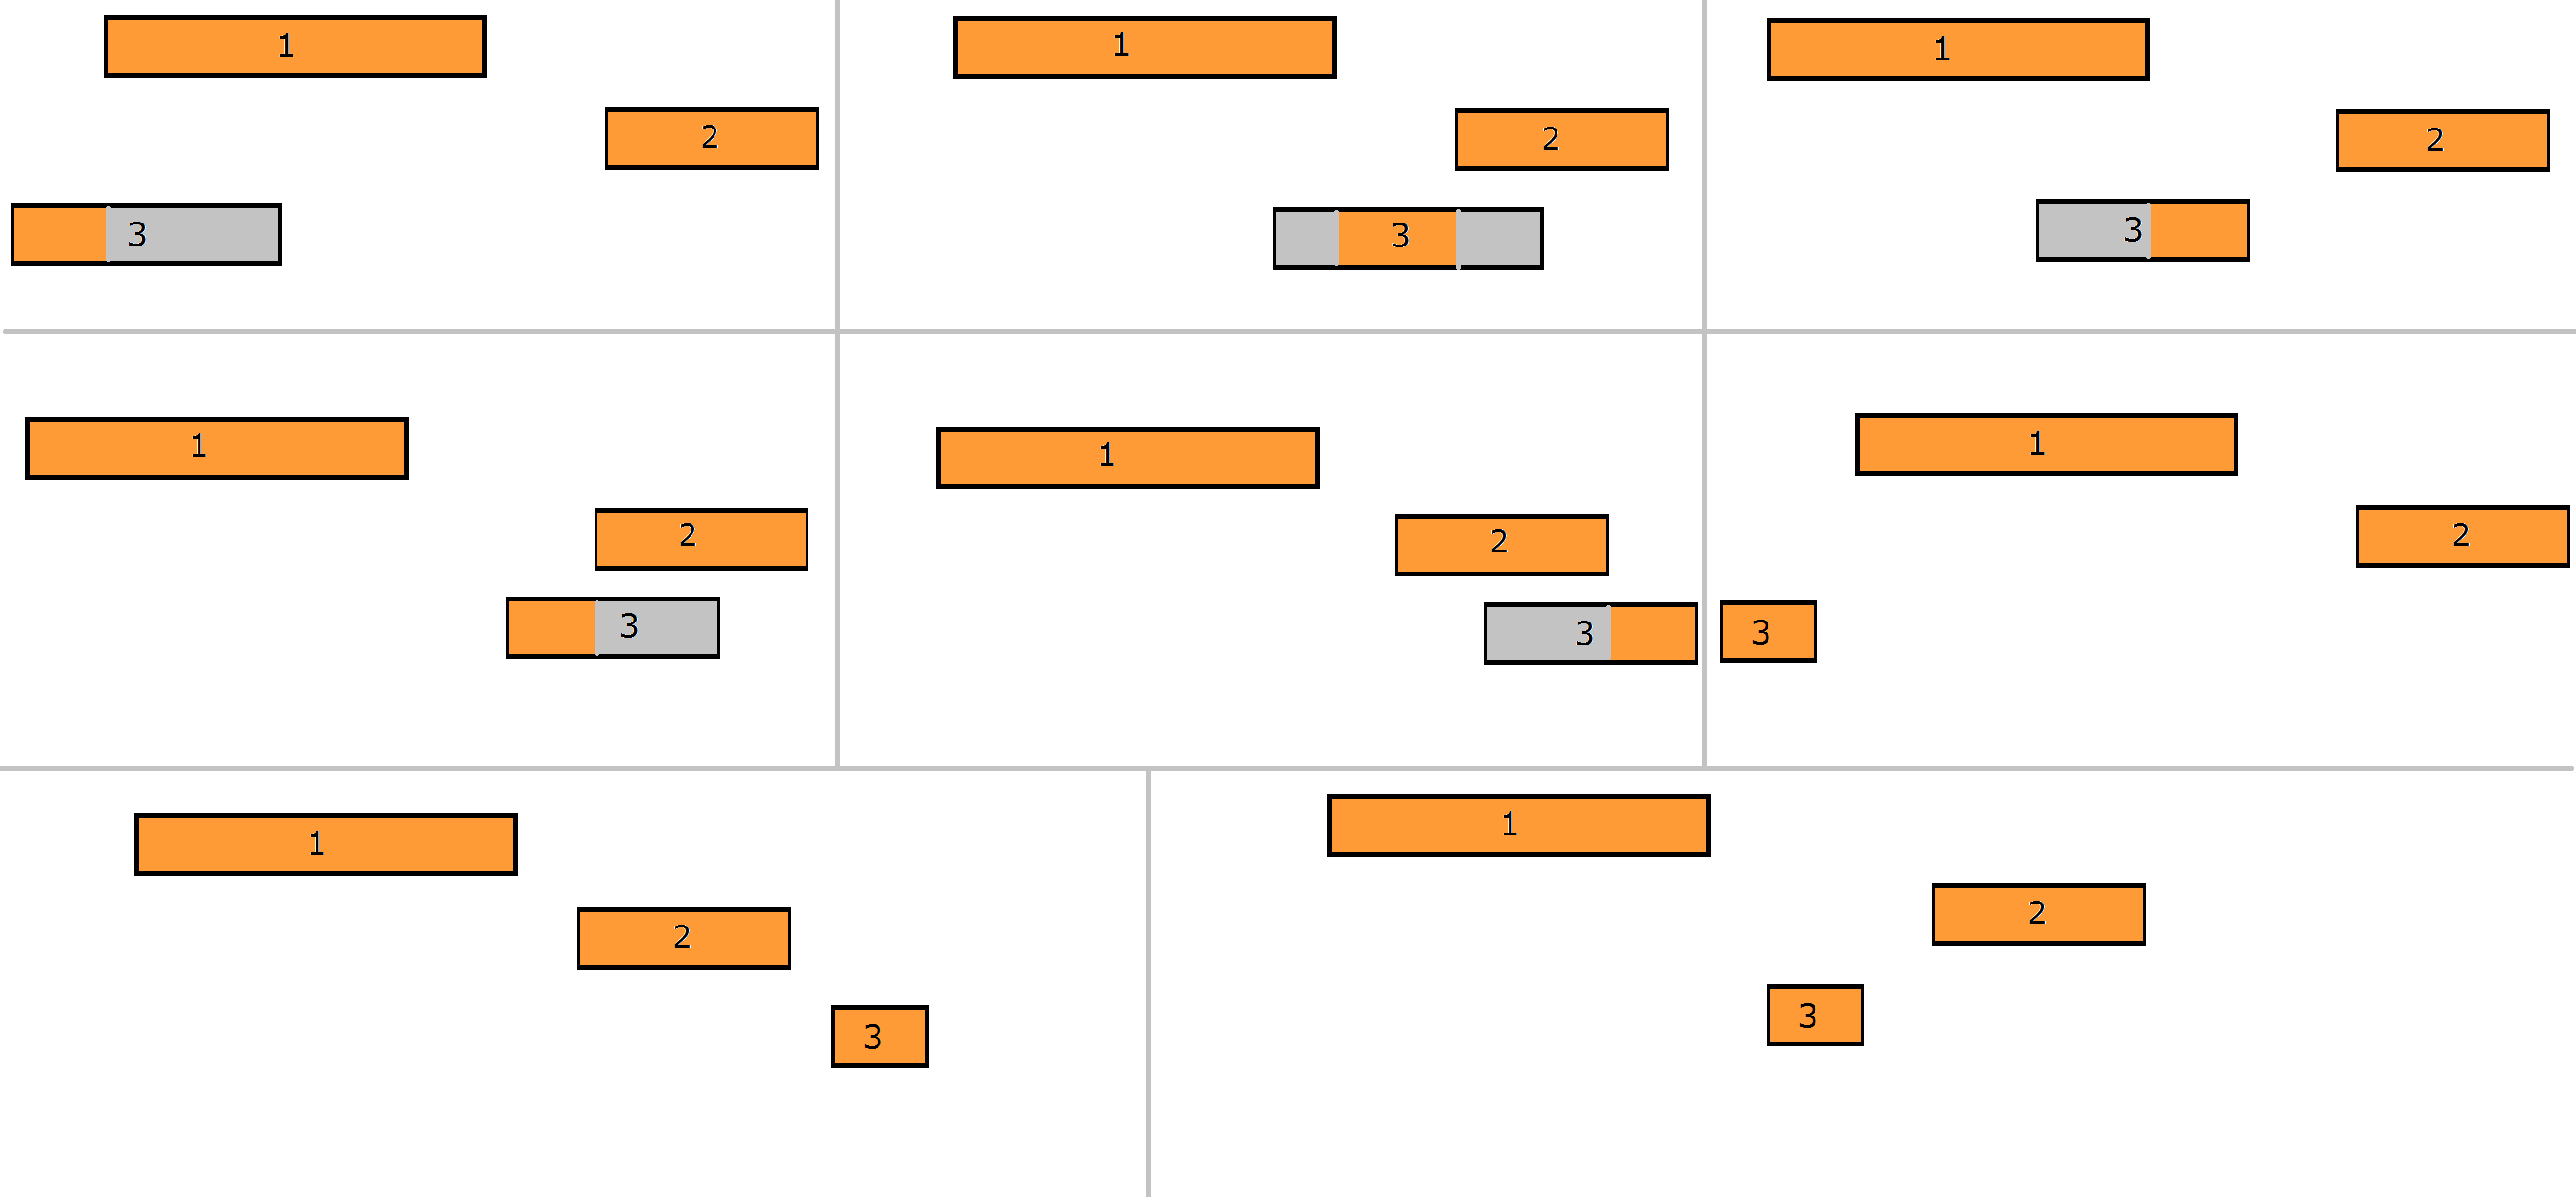
\includegraphics[scale=0.2]{imagenes/ej2/secuencias/Paso2/todos1.png}
% 	\caption{}
% 	\label{caballito}	
   \end{center}
 \end{figure}

Por consiguiente, el m\'aximo de intervalos que pueden a\~nadirse son tres, considerando siempre s\'olo dos pre-existentes, lo cual da un total de 5 que cumple: $2n-1$ $=$ $2$.$3-1$ $=$ $5$.\\

%Hasta el caso 3) se ve claramente que el m\'aximo n\'umero de intervalos es el propuesto (agregar un intervalo a izquierda y uno a derecha). Para el caso 4) hay que tener en cuenta que el paso anterior fue un caso de no solapamiento, es decir que si intercambiara la frecuencia que completa gaps con la no solapada, entonces entrar\'ia en el caso 2) o en el caso 3), verificando que a lo sumo se llega a \emph{2n-1} intervalos.\\

Si extendemos este c\'alculo para cualquier n, vamos a concluir que siempre la cantidad de intervalos va a estar acotada por $2n-1$ ya que se puede reducir el problema a cualquiera de las situaciones mencionadas.\\%\textcolor{red}{Habra que explicar un poco mas? O con esto basta?}


Partimos de la hip\'otesis de que los costos de las frecuencias eran todos distintos, lo cual nos asegura una soluci\'on \'unica con una cantidad \'unica de intervalos. Ahora, si consideramos que pueden existir dos (o m\'as) frecuencias, llamemos \emph{A} y \emph{B}, con el mismo precio podemos asumir indistintamente que \emph{A$<$B} o \emph{A$>$B} lo cual podr\'ia devolver intervalos distintos, pero siempre su cantidad va a estar acotada por lo mismo probado anteriormente: $2n-1$.\\

Una vez que ya acotamos la cantidad final de intervalos por $2n-1$, podemos proceder al an\'alisis de complejidad del algoritmo de Divide \& Conquer.\\

El algoritmo $divide$ particiona el problema en dos subproblemas m\'as chicos, en particular de la mitad de tamaño que el problema original, lo que implica que tiene complejidad \emph{T(n)=2T(n/2)+O(conquer)}.\\
\textcolor{red}{No hay que explicar medianamente de donde salio el 2T(n/2)?}\textcolor{blue}{Listo?}

Donde conquer va a recorrer, en el peor caso, dos vectores cuyas longitudes son $(2n-1)/2$ cada uno, y aplicar operaciones que toman $O(1)$ para cada una de ellas. El vector que va construyendo con el CS toma $O(2n-1)$ que es igual a $O(n)$. Estas complejidades se suman y por propiedades de O se obtiene $O(n)$.\\

Reemplazando en la ecuaci\'on obtenemos: \emph{T(n)=2T(n/2)+O(n)}. Vemos que es la misma ecuaci\'on de recurrencia que el algortimo de MergeSort, que por Teorema Maestro se deduce que tiene complejidad $O(n.log(n))$, como pretend\'iamos.

\newpage
\subsection{C\'odigo fuente}



	\begin{codesnippet}
	\begin{verbatim}
struct frecuencia{
    long int id;
    long int costo;
    long int principio;
    long int fin;
    bool operator< (const frecuencia& otro) const{
        if(costo == otro.costo){
            if(principio == otro.principio)
                return fin > otro.fin;
            return principio < otro.principio;
        }
        return costo < otro.costo;
    }
};
	\end{verbatim}
	\end{codesnippet}
	
		\begin{codesnippet}
	\begin{verbatim}
int main(int argc, char const *argv[]){
    chrono::time_point<chrono::system_clock> start, end;
    long int cantFrec;
    vector<frecuencia> frecuencias;
    //Leemos informacion del problema
    cin >> cantFrec;
    for (int i = 0; i < cantFrec; ++i){
        frecuencia actual;
        actual.id = i;
        cin >> actual.costo;
        cin >> actual.principio;
        cin >> actual.fin;
        if(actual.fin > actual.principio)
        frecuencias.push_back(actual);
    }
    start = chrono::system_clock::now();
    //Aplicamos el algoritmo
    vector<frecuencia> optimas = altaFrecuencia(frecuencias);
    vector<frecuencia>::iterator iter;
    //Calculamos el costo total (lo tuvimos en cuenta en la medicion de tiempos y complejidad)
    long int costoTotal = 0;
    for (iter = optimas.begin(); iter != optimas.end(); iter++){
        costoTotal += (iter->fin - iter->principio) * iter->costo;
    }
    end = chrono::system_clock::now();
    //Stdout pedido
    cout << costoTotal << endl;
    for (iter = optimas.begin(); iter != optimas.end(); iter++){
        cout << iter->principio << " " << iter->fin << " " << iter->id + 1 << endl;
    }
    cout << "-1" << endl;
    chrono::duration<double> elapsed_seconds = end-start;
    cout << "Tiempo: " << elapsed_seconds.count() << endl;
    return 0;
}
	\end{verbatim}
	\end{codesnippet}
	
	
		\begin{codesnippet}
	\begin{verbatim}
vector<frecuencia> altaFrecuencia(vector<frecuencia>& frecuencias){
    //Ordenamos el vector de menor a mayor costo de cada frecuencia
    sort(frecuencias.begin(), frecuencias.end());
    return divide(frecuencias, 0, frecuencias.size()-1);
}
	\end{verbatim}
	\end{codesnippet}

	
		\begin{codesnippet}
	\begin{verbatim}
vector<frecuencia> divide(vector<frecuencia>& frecuencias, long int comienzo, long int final){
    //Si tenemos dos o mas frecuencias, llamos a divide con cada una las mitades
    // y luego combinamos las soluciones
    if(final - comienzo > 0){
        vector<frecuencia> barata = divide(frecuencias, comienzo, (final+comienzo)/2);
        vector<frecuencia> cara = divide(frecuencias, ((final+comienzo)/2)+1, final);
        return conquer(barata, cara);
    }
    //Si solo hay una frecuencia,esta sera la forma mas barata y de maximo tiempo para transmitir
    else{
        vector<frecuencia> res;
        res.push_back(frecuencias[comienzo]);
        return res;
    }
}
	\end{verbatim}
	\end{codesnippet}
	
	
		\begin{codesnippet}
	\begin{verbatim}
vector<frecuencia> conquer(vector<frecuencia> barata, vector<frecuencia> cara){
    vector<frecuencia>::iterator iterCara = cara.begin(), iterBarata = barata.begin();
    vector<frecuencia> res;
    //mientras tenga frecuencias caras
    while(iterCara != cara.end()){
        // si todavia tengo baratas
        if(iterBarata != barata.end()){
            // si la cara empieza antes que la barata
            if(iterCara->principio < iterBarata->principio){
                // si la cara termina antes de que empiece la barata o al mismo tiempo
                if(iterCara->fin <= iterBarata->principio){
                    // la cara es parte de la solucion
                    res.push_back(*iterCara);
                    iterCara++;
                }
                // sino la cara empieza antes y termina despues del principio de la barata
                else{
                    // agrego el pedazo de cara que es solucion 
                    // y le digo que su nuevo principio es el fin de la barata
                    frecuencia antes;
                    antes.id = iterCara->id;
                    antes.costo = iterCara->costo;
                    antes.principio = iterCara->principio;
                    antes.fin = iterBarata->principio;
                    res.push_back(antes);
                    iterCara->principio = iterBarata->fin;
                }
            }
            // sino la barata empieza antes o al mismo tiempo que la cara
            else{
                // si la cara termina despues que la barata
                if(iterCara->fin > iterBarata->fin){
                    // si la cara intersecta con la barata, 
                    //le digo que su nuevo principio es el fin de la barata
                    if (iterCara->principio < iterBarata->fin)
                    iterCara->principio = iterBarata->fin;
                    // la barata es parte de la solucion
                    res.push_back(*iterBarata);
                    iterBarata++;
                }
                // si no salteo la cara, hay una o mas frecuencias para el tiempo 
                //en que se puede utilizar que son mas baratas
                else
                iterCara++;
            }
        }
        // sino agrego todas las caras restantes a la solucion
        else{
            if(iterCara->principio < iterCara->fin)
            res.push_back(*iterCara);
            iterCara++;
        }
    }
    //si me quede sin caras, agrego las baratas restantes a la solucion
    while(iterBarata != barata.end()){
        res.push_back(*iterBarata);
        iterBarata++;
    }
    return res;
}
	\end{verbatim}
	\end{codesnippet}
		
	
\newpage
\subsection{Experimentaci\'on}

\subsubsection{Constrastaci\'on Emp\'irica de la complejidad}



\begin{table}[htb]
\centering
\begin{tabular}[c]{|l|l|}

		\hline
n & Tiempo en segundos\\
		\hline
100	&	0.000415645\\
		\hline
150	&	0.00049622\\
		\hline
200	&	0.000595058\\
		\hline
300	&	0.000752836\\
		\hline
400	&	0.001029706\\
		\hline
500	&	0.001253788\\
		\hline
750	&	0.001757269\\
		\hline
1000	&	0.0023792\\
		\hline
1500	&	0.003352018\\
		\hline
2000	&	0.004313126\\
		\hline
3000	&	0.006464969\\
		\hline
5000	&	0.010964701\\
		\hline
6500	&	0.013377069\\
		\hline
8000	&	0.01643833\\
		\hline
9500	&	0.0197472\\
		\hline
10500	&	0.021750165\\
		\hline
11500	&	0.024404865\\
		\hline
12500	&	0.02591816\\
		\hline
		
		
		
	\end{tabular}
%\caption{Tabla muy sencilla.}
%\label{tabla:sencilla2}
\end{table}


  \begin{figure}[h!]
   \begin{center}
 	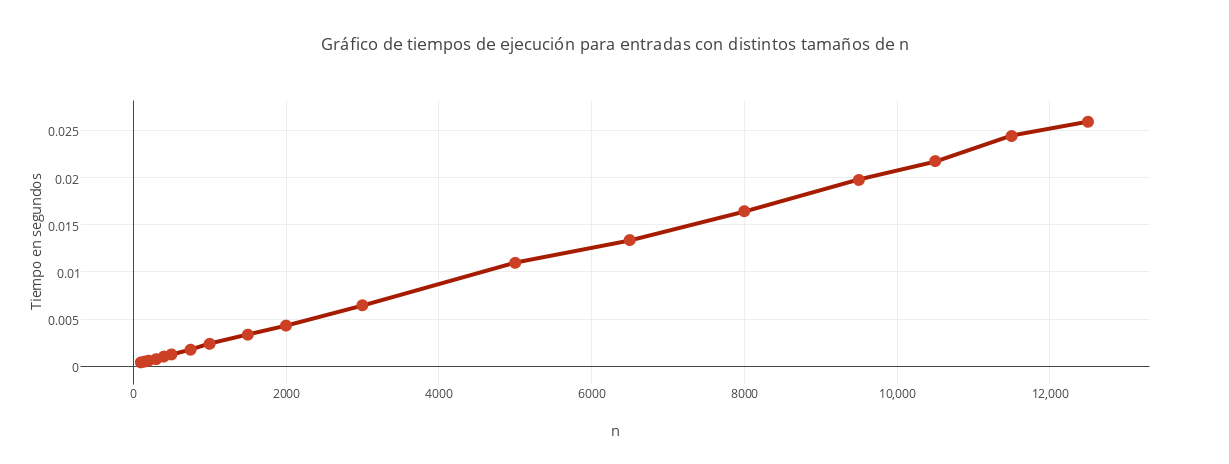
\includegraphics[scale=1.7]{imagenes/ej2/grafiquitos/graf1.png}
% 	\caption{}
% 	\label{caballito}	
   \end{center}
 \end{figure}
 \newpage
%   \begin{figure}[h!]
%   \begin{center}
% 	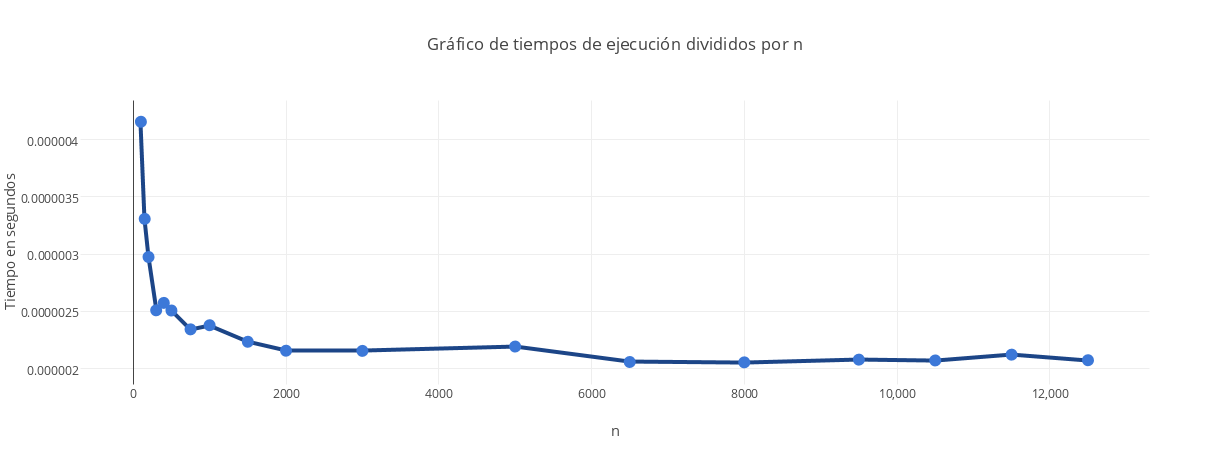
\includegraphics[scale=1.7]{imagenes/ej2/grafiquitos/graf2.png}
% 	\caption{}
% 	\label{caballito}	
%   \end{center}
% \end{figure}

\begin{table}[htb]
\centering
\begin{tabular}[c]{|l|l|}

		\hline
n & Tiempo en segundos dividido por log$_2$(n)\\ 
 	\hline
100	&	0.000207823	\\
 	\hline
 150	&	0.000228033	\\
	\hline
 200	&	0.000258605	\\
	\hline
 300	&	0.000303916	\\
	\hline
 400	&	0.000395727	\\
	\hline
 500	&	0.000464543	\\
	\hline
 750	&	0.000611211	\\
	\hline
 1000	&	0.000793067	\\
	\hline
 1500	&	0.001055391	\\
	\hline
 2000	&	0.0013066	\\
	\hline
 3000	&	0.001859288	\\
	\hline
 5000	&	0.002964258	\\
	\hline
 6500	&	0.003508359	\\
	\hline
 8000	&	0.00421162	\\
	\hline
 9500	&	0.004964447	\\
	\hline
 10500	&	0.005408889	\\
	\hline
 11500	&	0.006010017	\\
	\hline
 12500	&	0.00632627	\\
	\hline
  	
		
		
		
	\end{tabular}
%\caption{Tabla muy sencilla.}
%\label{tabla:sencilla2}
\end{table}
 
   \begin{figure}[h!]
   \begin{center}
 	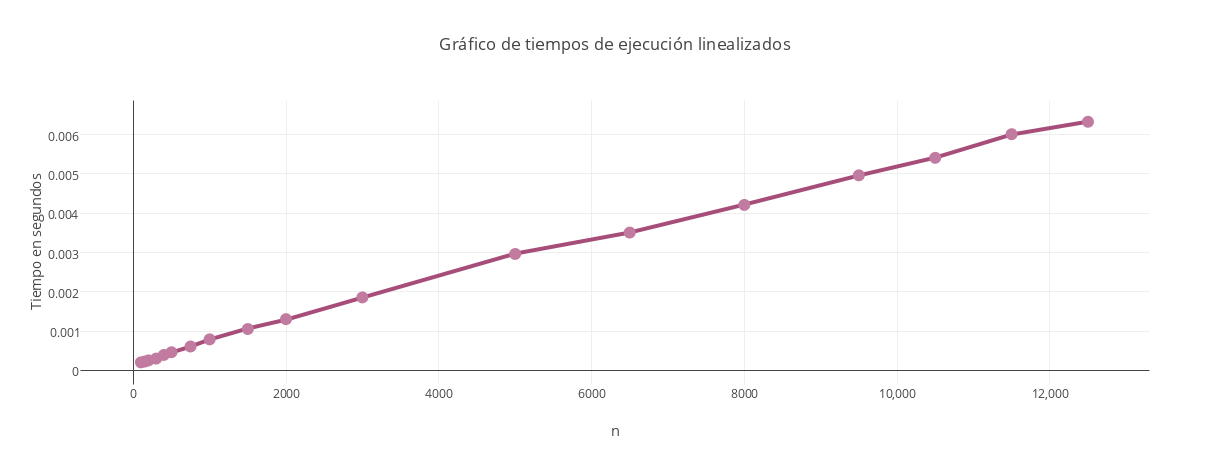
\includegraphics[scale=1.7]{imagenes/ej2/grafiquitos/graf3.png}
% 	\caption{}
% 	\label{caballito}	
   \end{center}
 \end{figure}
\newpage
\section{Problema 3: El se\~nor de los caballos}
\subsection{Descripci\'on de la problem\'atica}

En este problema, se presenta un tablero de ajedrez de tama\~no $nxn$, el cual cuenta con alguna cantidad de caballos ubicados en una posici\'on aleatoria del tablero. Lo que se quiere lograr es \emph{cubrir} todo el tablero. Un casillero se considera cubierto si hay un caballo en \'el o bien, si es una posici\'on en la cual alg\'un caballo existente puede moverse con un s\'olo movimiento. Para lograr este cometido, puede ser necesario agregar nuevas fichas \emph{caballo} al tablero. No existe un l\'imite en la cantidad de caballos para agregar, pero lo que se busca es dar una soluci\'on con la m\'inima cantidad de caballos posibles.\\


En la figura \ref{caballito} se pueden ver todas las casillas que est\'an cubiertas por un s\'olo caballo.


 \begin{figure}[h!]
   \begin{center}
 	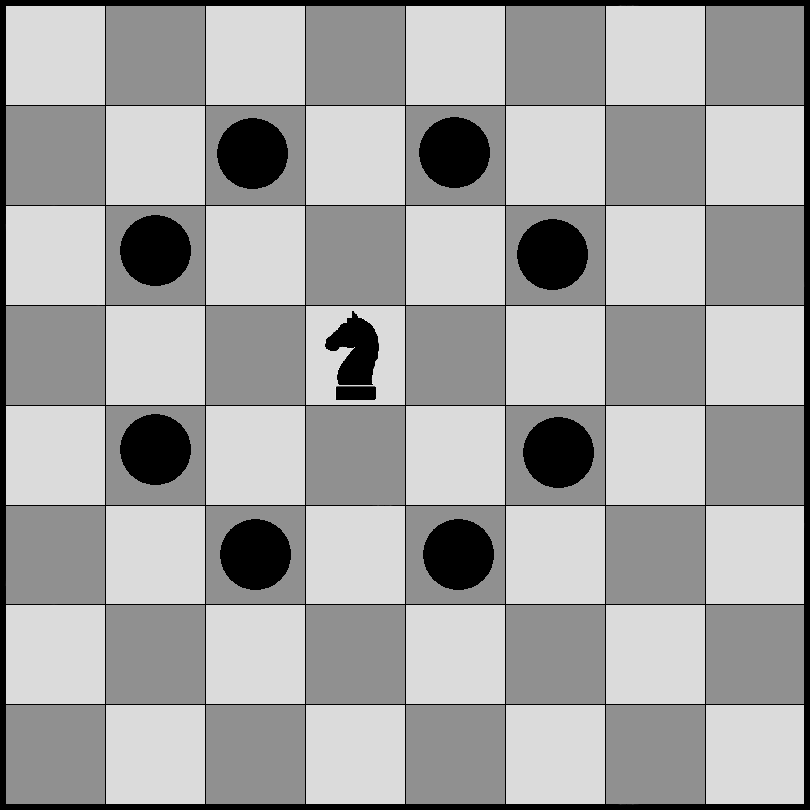
\includegraphics[scale=0.3]{imagenes/ej3/caballito.png}
 	\caption{Casillas que \emph{cubre} un caballo}
 	\label{caballito}	
   \end{center}
 \end{figure}



\newpage
\subsection{Resoluci\'on propuesta y justificaci\'on}
\textcolor{blue}{Esto va en algun lado?}\\
\textcolor{blue}{Ya no se ni donde van las cosas! JAJAJA}\\

Para la resoluci\'on de este ejercicio, se ped\'ia un algoritmo de backtracking. La soluci\'on que presentamos tiene inclu\'idas estrategias para que el algoritmo resuelva en un tiempo razonable los problemas medianos.\\

Vale aclarar que si el tablero ya estaba cubierto de antemano, simplemente hab\'ia que chequearlo, tomando $O(n^{2})$.\\

En primera instancia decidimos armar un algoritmo de backtracking "bobo", que revise todas las posibles combinaciones de tableros y nos devuelve la m\'as \'optima para este problema.\\

Simplemente se fija cu\'antos caballos necesita colocar para cubrir el tablero si no coloca un caballo en alguna posici\'on y luego se fija cu\'antos har\'an falta si lo pone en la misma posici\'on. Este m\'etodo de "fuerza bruta" tiene una complejidad de $O(2^{n^{2} - k})$ siendo n la dimensi\'on del tablero y k la cantidad de caballos preubicados. Esto es para cada posici\'on sin caballos, ver que pasa si tomo alguna de las dos posibles decisiones.\\

Para disminuir la cota de complejidad, se plantearon podas y estrategias, es decir, determinar si vale la pena o no seguir revisando alguna rama del \'arbol de soluciones que propone esta t\'ecnica de programaci\'on.\\

La primera poda fue la m\'as intuitiva, si tenemos una soluci\'on con k caballos extra agregados,  y analizando otra rama llegamos a tener que necesitar agregar un caballo a una subsoluci\'on de k-1 caballos (o sea que tendr\'ia k caballos), entonces no nos interesa seguir revisandola, pues tenemos una soluci\'on que es igual o m\'as \'optima con k caballos.\\

\textcolor{blue}{SHAMUSHO}\\

La segunda estrategia fue plantear si en alg\'un momento sab\'iamos que deb\'iamos agregar o no un caballo en un determinado casillero. Entonces, salteamos las k posiciones de los caballos preubicados y adem\'as salteamos aquellas posiciones que, estando atacadas, si le pusieramos un caballo, estar\'ian atancando a casilleros que ya est\'an siendo atacados por otros caballos.\\

\newpage

\subsection{An\'alisis de la complejidad}
\newpage

\subsection{C\'odigo fuente}
\newpage
\subsection{Experimentaci\'on}

\subsubsection{Constrastaci\'on Emp\'irica de la complejidad}
-Hacer lo que hicieron en clase\\
\newpage

\newpage

% \section{Objetivos generales}

% El objetivo de este Trabajo Práctico es ...


% \section{Contexto}

% \begin{figure}
%   \begin{center}
% 	
\includegraphics[scale=0.66]{imagenes/logouba.jpg}
% 	\caption{Descripcion de la figura}
% 	\label{nombreparareferenciar}
%   \end{center}
% \end{figure}


% \paragraph{\textbf{Titulo del parrafo} } Bla bla bla bla.
% Esto se muestra en la figura~\ref{nombreparareferenciar}.




%Habra que insertar el enunciado???
% %\section{Enunciado y solucion} 
% %\input{enunciado}

% \section{Conclusiones y trabajo futuro}

\end{document}

